\chapter{Human Exposure to Electromagnetic Fields}
\label{chap:human-exposure-to-emfs}

\section{Introduction to Electromagnetic Fields}
\Gls{em} field, in a classical sense, i.e. non-quantum, is a concept denoting smooth motions of charged particles through space.
In classical electrodynamics, oscillating charges produce variations in the electric, $\mathcal{E}$, and magnetic, $\mathcal{H}$, field in a continuous manner where, in that case, energy is viewed as being transferred continuously through a field between any two distinct points in space~\cite{Griffiths2017Introduction}.
A simple visual representation of a plane wave, whose value, at any moment, is constant through any plane that is perpendicular to a fixed direction in space~\cite{Brekhovskikh1980Waves}, is shown in \cref{fig:em_waves}.
% source: https://tex.stackexchange.com/a/229678
\begin{figure}[ht]
    \centering
    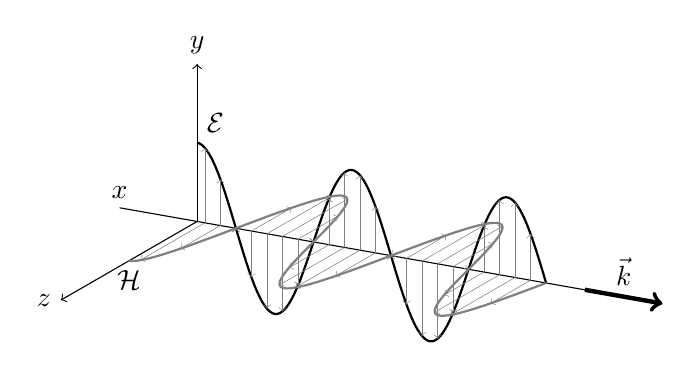
\begin{tikzpicture}[x={(-10:1cm)},y={(90:1cm)},z={(210:1cm)}]
        % Axes
        \draw (-1,0,0) node[above] {$x$} -- (5,0,0);
        \draw[->] (0,0,0) -- (0,2,0) node[above] {$y$};
        \draw[->] (0,0,0) -- (0,0,2) node[left] {$z$};
        % Propagation
        \draw[->,ultra thick] (5,0,0) -- node[above] {$\vec k$} (6,0,0);
        % Waves
        \draw[thick] plot[domain=0:4.5,samples=200] (\x,{cos(deg(pi*\x))},0);
        \draw[gray,thick] plot[domain=0:4.5,samples=200] (\x,0,{cos(deg(pi*\x))});
        % Arrows
        \foreach \x in {0.1,0.3,...,4.4} {
          \draw[->,help lines] (\x,0,0) -- (\x,{cos(deg(pi*\x))},0);
          \draw[->,help lines] (\x,0,0) -- (\x,0,{cos(deg(pi*\x))});
        }
        % Labels
        \node[above right] at (0,1,0) {$\mathcal{E}$};
        \node[below] at (0,0,1) {$\mathcal{H}$};
    \end{tikzpicture}

    \caption{Visual representation of a propagating plane wave in classical electrodynamics with $\vec k$ being the wave vector dictating the direction in which the wave propagates and is perpendicular to the wave-front \cite{Brekhovskikh1980Waves}.}
    \label{fig:em_waves}
\end{figure}

The number of oscillations per unit time is referred to as the frequency, $f$, of the field.
The quantum picture of \gls{em} fields is somewhat different.
Here, the moving charged particles are treated as ``quantum harmonic oscillators'' described via \gls{em} field tensors.

Mathematically, \gls{em} fields can be formulated within the Maxwell framework originally consisted of twenty scalar equations and subsequently reduced to four partial differential vector equations that encapsulate expressions for the relationship between fields and their sources in a symmetric form~\cite{Poljak2006Advanced}
\begin{align}
    \label{eqn:maxwell-faraday}
    \nabla \times \mathcal{E} &= -\frac{\partial \mathcal{B}}{\partial t},\\
    \label{eqn:maxwell-ampere}
    \nabla \times\mathcal{H} &= \mathcal{J} + \frac{\partial \mathcal{D}}{\partial t},\\
    \label{eqn:maxwell-gauss}
    \nabla \cdot \mathcal{D} & = \rho,\\
    \label{eqn:maxwell-gauss-magnetics}
    \nabla \cdot \mathcal{B} &= 0.
\end{align}
\Cref{eqn:maxwell-faraday} represents the differential form of the Faraday law which states that the time-varying magnetic flux density, $\mathcal{B}$, is the source of the rotating electric vector field, $\mathcal{E}$.
An extended differential formulation of the Ampere law is given in \cref{eqn:maxwell-ampere}.
It states that electric current density, $\mathcal{J}$, is the source of the rotating magnetic vector field, $\mathcal{H}$.
Furthermore, with an addition of displacement currents -- given by the time-varying electric flux density, $\mathcal{D}$, the consistency with the law of conservation of electric charge is achieved.
In \cref{eqn:maxwell-gauss}, the Gauss law, outlining the relationship between static electric fields and electric charges is given.
A static electric field points exclusively from positive towards negative charges with the net field outflow being proportional to the charge in a bounded volume of space.
On the other hand, the Gauss law for magnetism, which excludes the existence of magnetic monopoles -- the magnetic field is always solenoidal, is given in \cref{eqn:maxwell-gauss-magnetics}.

As the field propagates away from a source, it transfers
energy from its source to the surrounding space.
The general conservation of energy for a configuration consisting of electric and magnetic fields acting on charges is given by the Poynting theorem.
This theorem represents an energy balance indicating the rate of energy transfer (per unit volume) from a region of space is equal to the rate given by the work done on a charge distribution within the volume and the energy flux leaving that region reduced by the rate at which energy leaves the volume~\cite{Jackson1998Classical}.
It is written as~\cite{Durney1986Radiofrequency}
\begin{align}
    \label{eqn:poynting-theorem}
    \frac{\partial}{\partial t}\int_V \big( W_c + \frac{1}{2} \; \varepsilon \; \vec E \cdot \vec E^* + \frac{1}{2} \; \mu \; \vec H \cdot \vec H^* \big) \; \mathrm{d}V + \oint_S \big( \mathcal{E} \times \mathcal{H} \big) \; \mathrm{d} \vec S = 0.
\end{align}
In \cref{eqn:poynting-theorem}, $W_c$ represents energy of the charged particles (including both sources and losses) at a given point in the bounded volume, $V$.
Expressions $\frac{1}{2} \; \varepsilon \; \vec E^* \cdot \vec E$ and $\frac{1}{2} \; \mu \; \vec H^* \cdot \vec H$ are respectively energy stored in the electric and magnetic field, where $\varepsilon$ is the absolute permittivity and $\mu$ is the magnetic permeability.
The flow of energy through the surface, $S$, bounding the observed volume in a unit of time is defined as
\begin{align}
    \label{eqn:poynting-theorem-energy}
    \oint_S \big( \mathcal{E} \times \mathcal{H} \big) \; \mathrm{d} \vec S.
\end{align}
Within \cref{eqn:poynting-theorem-energy}, the time-varying vector field, i.e., the Ponyting vector,
\begin{align}
    \label{eqn:poynting-vector}
    \mathcal{P} = \mathcal{E} \times \mathcal{H},
\end{align}
represents the power density flow which defines the direction and amount of energy flow density at any point in space.

\section{Electromagnetic Radiation}
\gls{em} radiation is created due to periodic changes of electric and/or magnetic fields.
Depending on the periodicity and the overall \gls{em} power, different wavelengths of the \gls{em} spectrum are produced.
The frequency and wavelength are inversely proportional physical quantities whose proportionality constant is the propagation speed of \gls{em} waves in space.
In vacuum, where neither collisions nor any interaction with scatterers are captured, \gls{em} waves travel at the speed of light.
On the other hand, in lossy medium, the field travels at lower speed and can impact upon material which results in the interaction with atoms and molecules in that material.
Resulting effects depend both upon the transferred power and frequency/wavelength of the field as well as the physical properties and dimensions of the material which it interacts with.

\subsection{Non-Ionizing Electromagnetic Radiation}
With photon energy up to \SI{10}{\eV}, \gls{em} radiation is classified as non-ionizing since a single photon does not carry sufficient energy to ionize atoms or molecules by removing the most loosely bound corresponding electron.
It is grouped into different wavelength/frequency bands: \gls{uv} radiation (wavelengths of \SIrange[range-units=single,range-phrase=--]{100}{400}{\nm}), visible light (wavelengths of \SIrange[range-units=single,range-phrase=--]{400}{780}{\nm}), \gls{ir} radiation (wavelengths of \SIrange[range-units=single,range-phrase=--]{780}{1000}{\nm}), \gls{rf} \gls{em} fields (\SI{100}{\kHz} to \SI{300}{\GHz}), \gls{lf} (\SI{1}{\Hz} to \SI{100}{\kHz}) and static electric and magnetic fields.
On the other hand, even photons are electrically neutral, they still can lead to ionization of the matter indirectly through the photoelectric effect and the Compton effect.
It is generally accepted that indirectly ionizing radiation occurs for a photon's energy greater than \SI{10}{\eV} which is equivalent to the higher energy \gls{uv} part of the \gls{em} spectrum (wavelength of \SI{124}{\nm} or lower)~\cite{arpansa2022ionizing,Bulletin1999QuestionsAA}.
Thus, ionizing radiation falls into the high energy \gls{uv} spectrum, X-rays, and gamma rays.
Refer to \cref{fig:em_spectrum} for a full overview of the \gls{em} spectrum.
% source: https://tex.stackexchange.com/a/498765
\pgfdeclarehorizontalshading{visiblelight}{50bp}{% https://tex.stackexchange.com/a/348492/120853
    color(0bp)=(violet!25);
    color(8.33bp)=(blue!25);
    color(16.67bp)=(cyan!25);
    color(25bp)=(green!25);
    color(33.33bp)=(yellow!25);
    color(41.5bp)=(orange!25);
    color(50bp)=(red!25)
}%

\begin{figure}[ht]
    \centering
    \begin{tikzpicture}[%
            raylabel/.style={font=\scriptsize}
        ]
        \def\minexponent{-6}
        \def\maxexponent{6}
        \def\spectrumheight{9em}
    
        \pgfmathtruncatemacro{\nextminexponent}{\minexponent + 1}
    
        % Main foreach loop, drawing the wavelengths as powers of 10 in an alternating fashion: even on top, odd at bottom. Then connects them with help lines
        \foreach [count=\i, remember=\exponent as \previousexponent, evaluate=\i as \currentposition using int(\i/2)] \exponent in {\minexponent, \nextminexponent, ..., \maxexponent}{
            \ifodd\exponent
                \def\height{0}
            \else
                \def\height{\spectrumheight}
            \fi
    
            % Anchor at baseline to get all nodes on same baseline.
            % https://tex.stackexchange.com/questions/133227/how-to-align-text-in-tikz-nodes-by-baseline#comment300863_133227
            \node[anchor=base] (WAVELENGTH_\exponent) at (\exponent, \height) {\contour{white}{\num{e\exponent}}};
    
            \ifnum\i > 1
                \ifodd\i
                    \node (LABEL_\currentposition)
                        at ($(WAVELENGTH_\exponent)!0.5!(WAVELENGTH_\previousexponent)$)
                        {};% This is left as a node as opposed to coordinate: fill it out with '\currentposition' for debugging
                \else
                    % Do not draw connection at exponent 1:
                    \pgfmathparse{\exponent != 1}% \pgfmathparse stores result (0 or 1) in macro \pgfmathresult
                    \ifnum\pgfmathresult = 1
                        \draw[help lines]
                            (WAVELENGTH_\previousexponent) --(WAVELENGTH_\exponent)
                            node[midway] (CONNECTION_\currentposition) {}% This is left as a node as opposed to coordinate: fill it out with '\currentposition' for debugging
                            coordinate[at start] (CONNECTION_\currentposition_START)
                            coordinate[at end] (CONNECTION_\currentposition_END);
                    \fi
                \fi
            \fi
        }
    
        % Create an arrow shape that fits around all relevant nodes, but do not draw it.
        % Draw it manually later to leave out the 'bottom' of the arrow.
        % We still need this invisible arrow for lining up of coordinates
        \node[
            single arrow,
            single arrow head extend=0pt,
            single arrow tip angle=150,% Inner angle of arrow tip
            fit={([xshift=-3em]CONNECTION_1_START)(CONNECTION_1_END)(CONNECTION_\maxexponent_START)([xshift=5em]CONNECTION_\maxexponent_END)},
            inner sep=0pt
        ]
        (ARROW) {};
    
        \node[align=center] (THERM) at ([yshift=3em]WAVELENGTH_1|-ARROW.after tail) {thermal\\effects};% Only works because exponent 1 is between -1 and 3
        \draw (THERM) -| ([yshift=-1.5em]WAVELENGTH_-1|-THERM);
        \draw (THERM) -| ([yshift=-1.5em]WAVELENGTH_3|-THERM);
    
        % On background layer so already drawn arrow and scale lines cover it up nicely
        \begin{scope}[on background layer]
            \node[
                inner sep=0pt,
                outer sep=0pt,
                fit={([xshift=-2.2em]WAVELENGTH_0|-ARROW.after tail)([xshift=-2.2em]WAVELENGTH_1|-ARROW.before tail)}, shading=visiblelight]
                (SMALL_VISIBLE_LIGHT) {};
    
            \shade[
                left color=white,
                right color=violet!25,
                middle color=violet!5,
                outer sep=0pt
                ]
                (CONNECTION_3_START) -- (CONNECTION_3_END) -- ([xshift=\pgflinewidth]SMALL_VISIBLE_LIGHT.south west) -- ([xshift=\pgflinewidth]SMALL_VISIBLE_LIGHT.north west) -- cycle;
    
            \shade[
                left color=red!25,
                right color=white,
                middle color=red!5,
                outer sep=0pt,
                ]
                (CONNECTION_5_START) -- (CONNECTION_5_END) -- ([xshift=-\pgflinewidth]SMALL_VISIBLE_LIGHT.south east) -- ([xshift=-\pgflinewidth]SMALL_VISIBLE_LIGHT.north east) -- cycle;
        \end{scope}
    
        % Some labels can be drawn automatically at the designated label coordinates:
        \foreach [count=\i] \label in {
                {gamma\\rays},
                {X-rays},
                {},%Skip this one
                {\gls{ir}}
            }{
                \node[raylabel, align=center] at (LABEL_\i) {\label};
            }
    
        % These do not fit the loop and are drawn manually:
        \node[raylabel, anchor=north] at ([yshift=-3.85em]$(WAVELENGTH_-2)!0.45!(WAVELENGTH_0)$) {\gls{uv}};
    
        \node[raylabel, fill=white, align=center] at (CONNECTION_6) {\gls{rf}\\radiation};
    
        \node[raylabel, right=3em of CONNECTION_6, align=right] {\gls{lf}\\radiation};
    
        \node[raylabel, left=1em of CONNECTION_1, align=left] {cosmic\\rays};
    
        \node[
            draw,
            fill=black!20,
            below=4em of SMALL_VISIBLE_LIGHT,
            align=center,
            label=above:{\textbf{visible light}}
            ] (FULL_VISIBLE_LIGHT) {%
            \pgfspectra[width=13em,height=3em]\\%pgfspectra also has a builtin axis which of course much better than this terrible approach, but it is in nanometer
                {\SI{0.40}{} \hfill \SI{0.48}{} \hfill \SI{0.58}{} \hfill \SI{0.68}{} \hfill \SI{0.78}{\um}}
        };
    
        % Draw 'magnifying' trapeze, on background so it is covered by scale labels
        \begin{scope}[on background layer]
            \filldraw[help lines, fill=black!10] (FULL_VISIBLE_LIGHT.north east) -- (SMALL_VISIBLE_LIGHT.south east) -- (SMALL_VISIBLE_LIGHT.south west) -- (FULL_VISIBLE_LIGHT.north west) -- cycle;
        \end{scope}
    
        % Draw around arrow manually, leaving its tail open
        \draw[draw, thick] (ARROW.after tail) -- (ARROW.before head) -- (ARROW.before tip) -- (ARROW.tip) -- (ARROW.after tip) -- (ARROW.after head) -- (ARROW.before tail);
    \end{tikzpicture}
    
    \caption{Diagram of \gls{em} spectrum distribution as a function of wavelengths.}
    \label{fig:em_spectrum}
\end{figure}


By acting upon material in lossy space, non-ionizing \gls{em} waves transfer kinetic energy to surrounding bounded atoms and molecules in the material causing them to vibrate more rapidly.
This effect is accompanied by an increase in the temperature of the affected area, but it occurs only if wavelength of incident electromagnetic waves are of the same order of magnitude as the dominant dimension of the material being irradiated.
To put it in a perspective, \gls{lf} radiation has very long wavelengths (order of a thousand kilometres or more), \gls{rf} radiation have wavelengths of between \SI{1}{} and \SI{100}{\m}, with microwaves being about \SI{1}{\cm} long.
Thus, heating of biological tissue is the most prevalent in microwave spectrum and towards the lower energy part of \gls{uv} spectrum, see \cref{fig:em_spectrum}.

\subsection{Foundational Principles of Non-Ionizing Electromagnetic Radiation Effects on Tissue}
\label{sec:principles}
Conditioned by the interaction of non-ionizing radiation and biological tissue, a biological effect can be described as any biological, physical, or chemical change induced in this tissue~\cite{ICNIRP2020Principles}.
Living organisms have repair and feedback mechanisms intended primarily for preservation of homeostasis.
Once upper threshold limits in the capacity of these mechanisms are exceeded, adverse health effects may occur.
In some cases, the difference between the biological and adverse health effect is not clear as it may vary significantly upon individual's perception and sensitivity.
For this reason, adverse health effects are distinguished from other biological effects based on the World Health Organization definition of health: ``Health is a state of complete physical, mental and social well-being and not merely the absence of disease or infirmity''~\cite{WHO2022Health}.
If a biological perception appears as a consequence of non-ionizing radiation (e.g. tingling sensation~\cite{Saunders2007neurobiological}, magnetophosphenes~\cite{Lövsund1980Magnetophosphenes}, microwave hearing~\cite{Frey1962Human}), and it does not have consequences on the health of an individual, then it is not considered an adverse health effect~\cite{ICNIRP2020Principles}.

Interaction effects between non-ionizing radiation and biological tissue are roughly classified into the thermal and non-thermal category.
Low frequency \gls{rf} radiation up to \SI{100}{\kHz} usually pertains to non-thermal effects, e.g., nerve stimulation, while \gls{rf} radiation above \SI{10}{\MHz} is exclusively associated with thermal effects by means of tissue temperature rise.
The overview of the non-ionizing \gls{em} spectrum and the effects on biological tissue is outlined in \cref{tab:interaction-mechanism}.
\begin{table}[ht]
    \centering
    \caption{Summary of non-ionizing radiation effects on biological tissue.}
    \label{tab:interaction-mechanism}
    \resizebox{\textwidth}{!}{%
        \begin{tabular}{|c|c|c|}
            \hline \rowcolor[HTML]{EFEFEF}exposure to  & frequency range & \cellcolor[HTML]{EFEFEF}effect of interaction \\ \hline static magnetic fields & \SI{0}{\Hz} & induced electric fields and current \\
            \hline \gls{lf} radiation & \SI{1}{\Hz} to \SI{100}{\kHz} & stimulation of excitable cells \\
            \hline & \SI{100}{\kHz} to  \SI{10}{\MHz} & stimulation of excitable cells and tissue heating \\
            \cline{2-3} \multirow{-2}{*}{\gls{rf} radiation} & \SI{100}{\MHz} to \SI{300}{\GHz} & \\
            \cline{1-2} \gls{ir} radiation & \SI{300}{\GHz} to  $\sim$ \SI{400}{\THz} & \\
            \cline{1-2} visible light & $\sim$ \SI{400}{\THz} to  $\sim$ \SI{790}{\THz} & \\
            \cline{1-2} low energy \gls{uv} & above \SI{790}{\tera\Hz} & \multirow{-4}{*}{tissue heating} \\
            \hline
        \end{tabular}%
    }
\end{table}
Exposure to \gls{em} fields induces electric fields within tissue, which can stimulate any excitable cells of that tissue up to \SI{10}{\MHz}~\cite{Saunders2007neurobiological}.
Low frequency, pulsed \gls{em} fields of sufficient intensity may lead to the change in permeability of cell membranes and subsequent deformation of intracellular structures if the duration is shorter than the charging time of the outer membrane~\cite{Joshi2010Critical}.
Increasing the frequency, heating effects predominate and the likelihood of nerve stimulation drastically decreases.
However, evidences on the existence of non-thermal effects above \SI{100}{\MHz} exist~\cite{Romanenko2017interaction} and are usually manifested as changes in the activity of cell membranes and non-selective channels, transmembrane potentials and the cell cycle.
Since there is no scientific consensus of their adverse health effects, they fall out of the scope of this work.
It is nevertheless important to note that in~\cite{Fröhlich1968Long}, theoretical predictions of the existence of megahertz to terahertz oscillations in the living cells were postulated and have sparked great interest in risks and potentials of the interaction of external \gls{em} fields and tissues.
Biological effects at physiological levels and at cellular and molecular levels have been reviewed extensively in~\cite{Pakhomov1998Current,Zhadobov2011Millimeter}.
Authors of the latter study argue that even though there are some arguments in favor of possible interactions of high frequency \gls{em} waves, especially at \gls{mmw}, with living organisms that exclude direct and indirect thermal effects, e.g., therapeutic applications~\cite{Ziskin2006Physiological}, it is unclear if these effects can be fully explained without placing them in the thermodynamics framework.

\section{Radio-Frequency Electromagnetic Radiation Protection}
With the development and widespread deployment of electronic systems, humans are increasingly being exposed to artificial \gls{em} fields~\cite{Hirata2021Assessment}.
Most consumer electronics fall into the \gls{rf} portion of the \gls{em} spectrum as they are usually based on the services of communication and wireless transmission of information and recently, on a larger scale, on wireless power transfer.
To ensure safe use of such devices, various international bodies set guidelines or standards for limiting exposure to \gls{em} fields.
\Gls{icnirp} and \gls{ieee} International Commitee on \gls{em} Safety prescribe exposure limits through guidelines~\cite{ICNIRP2020Guidelines} and standards~\cite{IEEE2019Standard}, respectively, both for people in restricted environments and for the general public.

A high degree of protection against adverse health effects is ensured by respecting the frequency and exposure scenario dependent limits to both short- and long-term, continuous and discontinuous \gls{rf} \gls{em} fields~\cite{ICNIRP2020Guidelines,IEEE2019Standard}.
The limits are derived upon published scientific literature pertaining to the effects of \gls{rf} \gls{em} field exposure on biological systems and tissues that is classified as potentially harmful.
These limits are subsequently identified as adverse health effect thresholds~\cite{ICNIRP2020Guidelines} (or exposure limits~\cite{IEEE2019Standard}).
Additionally, reduction factors~\cite{ICNIRP2020Guidelines} (or safety margins~\cite{IEEE2019Standard}) are applied to the resultant thresholds/limits or operational threshold/limits if no direct thresholds/limits can be explicitly obtained.
Reduction factors (or safety margins) account for feature variability of individuals as well as variations in the exposure setup, environment, etc.

Now, the threshold values, incorporating reduction factors (or safety margins), are expressed in terms of \gls{br}s~\cite{ICNIRP2020Guidelines} (or \gls{drl}s~\cite{IEEE2019Standard}).
They relate to physical dosimetric quantities, either peak or averaged in time and space, that are well correlated with occurrence of harmful impact as a result of \gls{rf} \gls{em} exposure.
To facilitate the assessment of exposure in situations where the aforementioned physical quantities are difficult to measure, \gls{rl}s~\cite{ICNIRP2020Guidelines} (or \gls{erl}s~\cite{IEEE2019Standard}) are derived upon \gls{br}s (or \gls{drl}s) under worst-case exposure conditions to acquire high degree of conservatism and to provide a more-practical means of demonstrating compliance with the guidelines (or standards).

\subsection{Brief Historical Overview}
Ever since the first commercial radio station was put in operation and started broadcasting, there has been a public interest in assessment of human exposure to \gls{rf} \gls{em} radiation.
Serious endeavors in the scientific investigation of the interaction of \gls{em} waves of \gls{rf} spectrum and human tissue were initiated during the 20s of the last century given the rapidly expanded use of \gls{rf} diathermy for therapeutic tissue heating~\cite{Kovacs1945Electrotherapy}.

In the early 50s, the US Department of Defense put in operation a large number of high-power \gls{rf} transmitters to enable the advanced use of wireless communications and radar systems.
As most of the transmitters were operated in close proximity to personnel, there existed a concern about possible adverse health effects.
The Tri-Services Program (1956–1960) was put in operation and had the main goal to examine the potential impact of radiated fields on the human body~\cite{Lin1994Early}.

Although research in this area was brought to a higher level of quality~\cite{Guy1971Analyses} during the 70s, there was a growing distrust within the general population due to the increasing number of wireless electronic devices operating in the close proximity of human body whose safety was questionable due the chronic lack of concrete limits and regulations defined on the basis of rigorously verified scientific facts, but also the growing number of controversies~\cite{Foster2022Three}.
As a response, more and more computational dosimetry studies were published, mostly considering far-field exposure to plane wave radiation given the state of the technology at the time.
This culminated with publication of a series of dosimetry handbooks sponsored by the U.S. Air Force~\cite{Durney1986Radiofrequency}.

At the same time, comprehensive studies of
environmental RF fields in urban environments underwent proliferation~\cite{Tell1976Measurement}, and, to date, numerous surveys have measured environmental \gls{rf} fields from diverse technologies, e.g., \gls{rf} transmitters, base stations, mobile phones, etc., in different conditions and exposure scenarios~\cite{Jalilian2019Public}.
The first set of the formal \gls{rf} safety standards in U.S. were published during the late 60s from which the \gls{ieee} family of exposure standards, denoted C95.1-\textit{x}, where \textit{x} corresponds to the year of publication, arose.
This early limits were usually expressed in terms of the power density incident to the body and were based on canonical models predicting whole-body heating.
Subsequently, over the years, the development of international, often independent, regulatory bodies, including \gls{ansi}, \gls{icnirp}, \gls{ieee}, etc., has evolved.
Refer to~\cite{Roach2009Radiofrequency} for a more comprehensive historical background.

\Gls{icnirp}, an independent international organization, introduced generally similar guidelines; a history of the development of the organization and its guidelines are available elsewhere, e.g., in~\cite{Repacholi2017history}.
Although over the years there were significant discrepancies between \gls{ieee} C.95.1-\textit{x} standards and \gls{icnirp} guidelines, with the latest updates in 2019 and 2020, respectively, the harmonization between two sets of limits has mostly been achieved.
It is reported in~\cite{Foster2022Three} that ``a great deal since the days of the Tri-Services Program has been learned and major technical advances in exposure assessment and dosimetry have been reached''.
This includes the high-fidelity \gls{em} simulation software for computational dosimetry, large-scale, image-based libraries of 3-D human and animals models adapted to \gls{em} simulations, high-quality, commercially available instruments for accurate \gls{rf} exposure assessment, etc.

During the last decade, research has at least doubled on all fronts: from experimental to epidemiological to dosimetric/technical studies.
However, the greatest progress can be seen in the quality and number of published studies carried out in computational dosimetry research, the main idea of which is the realization of precise simulations at high frequencies in the near field~\cite{Diao2021Effect}.
In 2021, in total $N = $ 375 studies related to computational dosimetry have been published concerning the exposure to \gls{rf} \gls{em} waves and/or mobile communications in general (see \cref{fig:research_compilation_2021}), which is more than a double compared to the number of published experimental studies ($N = $ 140).
\begin{figure}[ht]
    \centering
    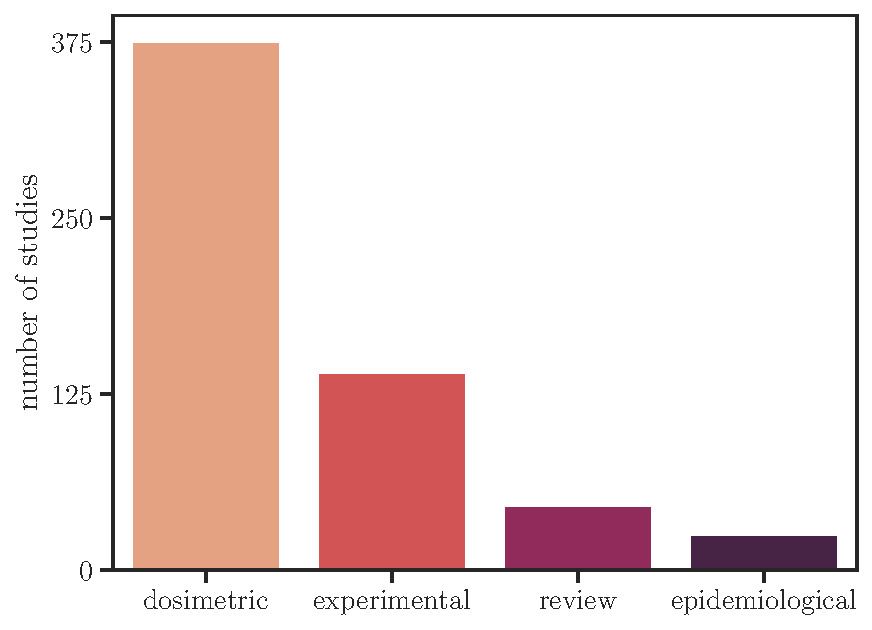
\includegraphics[width=0.8\textwidth]{artwork/research_compilation_2021.pdf}
    \caption{Papers published in 2021 related to research on bioeffects of \gls{rf} fields and/or mobile communications. Compiled from the database of publications at \url{emf-portal.org}.}
    \label{fig:research_compilation_2021}
\end{figure}
The reason for this is the market breakthrough of new wireless communication devices, primarily based on the \gls{5g} cellular technology, which, in addition to utilization of higher parts of the \gls{rf} spectrum compared to preceding generations, employs \gls{mimo} antennas and beam-steering~\cite{Andrews2014What}.
Considering the hard-to-maintain control conditions of the laboratory and expensive equipment, especially at \gls{mmw}, there is a dearth of accurately assessed and adequate experimental data.
The available experimental studies do not provide sufficient information for a meaningful safety assessment~\cite{Simkó20195G}.
Additionally, the advent of numerical methods~\cite{Poljak2018On}, e.g., \gls{fdtd}, \gls{fem}, \gls{bem}, \gls{mom}, etc., computing power and its overall availability, facilitated by the publicly available, highly-accurate databases on the dielectric properties of numerous human and animal tissues~\cite{Gabriel1996Compilation} has enabled progress in computer dosimetry and computational bioelectromagnetics in general.
The evolution of research from 1950 to 2021 in the field of \gls{rf} and/or mobile communications exposure assessment and dosimetry is visualized in \cref{fig:research_compilation}.
\begin{figure}[ht]
    \centering
    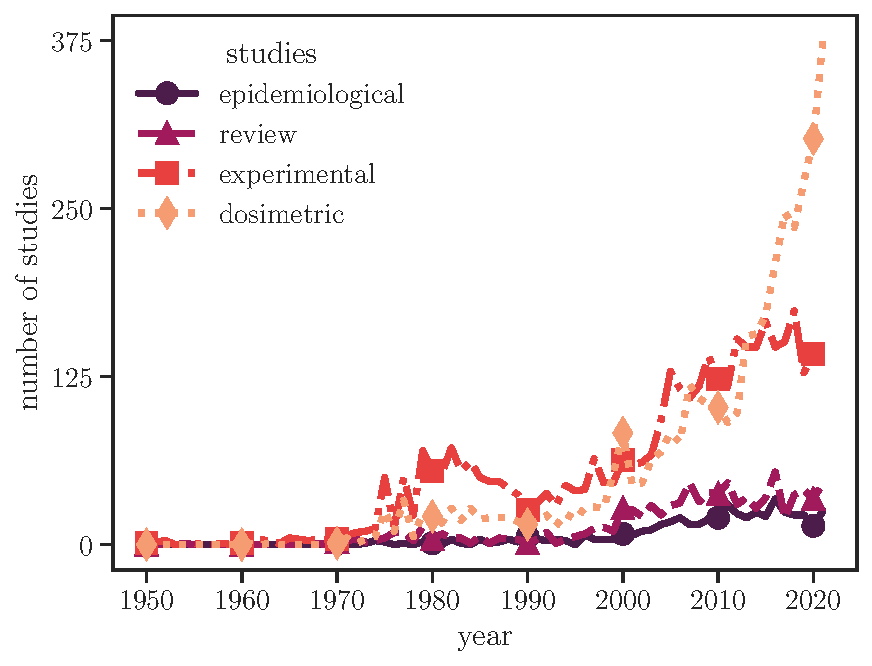
\includegraphics[width=0.8\textwidth]{artwork/research_compilation.pdf}
    \caption{Papers published over years from 1950 to 2021 related to research on bioeffects of RF fields and/or mobile communications. Compiled from the database of publications at \url{emf-portal.org}.}
    \label{fig:research_compilation}
\end{figure}

\subsection{Scientific Basis for Limiting Radio-Frequency Exposure}
As pointed out in the previous section, the main component of absorbed \gls{em} fields inside the body is the electric field.
Below \SI{10}{\MHz}, induced electric fields may stimulate nerves and, in rare occasions, cause dielectric breakdown of biological membranes~\cite{Swicord2008Has}.
Such and similar effects are defined as non-thermal and can be classified into four groups: resonance mechanisms, coupling with non linear systems, effects due to the direct action of electric and magnetic fields, and cooperative mechanisms due to interactions among several membrane components~\cite{DInzeo200dDeliverable}.
Above \SI{100}{\kHz}, the result of the interaction between induced electric fields and polar molecules or free charges within the exposed body is the kinetic energy.
It makes the polar molecules to rotate and oscillate around their center, while charges to form the electric current.
Increased kinetic energy leads to more frequent interaction with other polar molecules and charged particles, which ultimately causes conversion of kinetic into thermal energy~\cite{Foster2018Modeling}.

In order to evaluate the heating effects, it is important to quantify the absorbed \gls{em} power within exposed tissue.
It is generally considered that below \SI{6}{\GHz}, \gls{em} fields penetrate deep, whereas above this frequency, the power is dissipated mostly across the surface of the exposed tissue~\cite{Ziskin2018Tissue}.
The power transmission coefficient and power penetration depth into the uniform half plane of tissue with dielectric properties of dry skin as frequency-dependent functions are shown in \cref{fig:penetration_depth}.
\begin{figure}[ht]
    \centering
    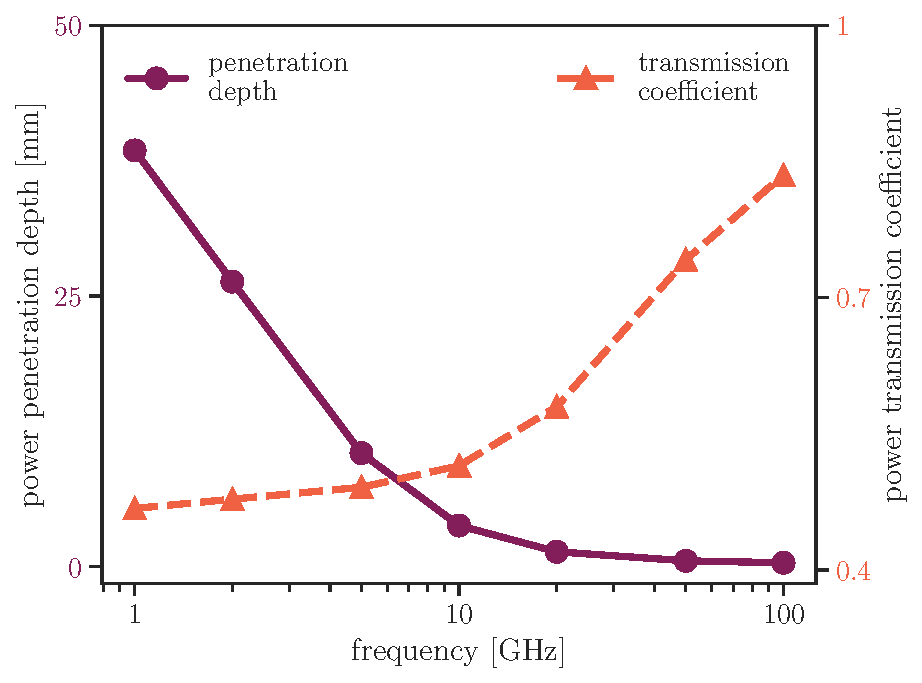
\includegraphics[width=0.8\textwidth]{artwork/penetration_depth.pdf}
    \caption{Power transmission coefficient and power penetration depth into dry skin as functions of frequency.}
    \label{fig:penetration_depth}
\end{figure}
Dielectric properties of dry skin are taken from~\cite{Gabriel1996Compilation}.
Power penetration depth into the tissue is defined
as the distance beneath the surface at which the power density has fallen to a factor of $1/e$ below that at the surface -- one-half of the more commonly reported wave penetration depth~\cite{Foster2016Thermal}.

Both guidelines and standards set (operational) threshold levels to restrict temperature rise rather than absolute temperature as it is dependent on many factors that are not conditioned by exposure to \gls{rf} \gls{em} fields.
Such factors, e.g., sex, age, thermoregulation, that are subject to inter-individual features together with additional confounding variables as surrounding temperature, clothing, and work rate are out of the scope of guidelines/standards.

Temperature rise can be further differentiated to steady-state and brief temperature rise.
Steady-state temperature rise allows time for heat to dissipate over a larger tissue mass and for thermoregulatory processes to become active.
Steady-state rise of body core temperature is generally limited to \SI{1}{\celsius} although there are no scientific evidences of adverse health effects in the event of even greater temperature increase.
Due to the limited literature available, steady-state temperature rise of \SI{1}{\celsius} has been adopted in a conservative manner as it triggers significant physiological changes, e.g., thermoregulatory responses~\cite{Heuvel2017independent} which are not represented as adverse health effects.

Additionally, steady-state local temperature rise is defined to account for specific exposed body regions such as the head and torso, or limbs.
It is accepted that local temperature rise should be limited to \SI{5}{\celsius} for regions  containing tissue with normothermal temperature in the \SIrange[range-units=single,range-phrase=--]{33}{36}{\celsius} range.
For regions with higher normothermal temperature in the \SIrange[range-units=single,range-phrase=--]{36}{38.5}{\celsius} range, e.g., tissues in the head, eyes, abdomen, thorax, pelvis, etc., local temperature rise should be limited to \SI{2}{\celsius}.
These limits are based on the experimental human studies~\cite{Walters2000Heating} given the fact that damage may occur at tissue temperature of \SIrange[range-units=single,range-phrase=--]{41}{43}{\celsius}~\cite{Dewhirst2003Basic} with the likelihood and severity of damage increasing with the increase of exposure time~\cite{ICNIRP2020Guidelines}.

Finally, rapid temperature rise can result in heterogeneous temperature distribution over mass or surface of the exposed tissue before thermoregulatory responses become active that allow heat dissipation within the tissue~\cite{Foster2016Thermal,Foster2017Thermal,Laakso2017Human,Kodera2018Brief}. This will be discussed in more detail in the following sections.

\subsection{Basic Restrictions}
\Gls{br}s/\gls{drl}s (from now on in the text only ``\gls{br}'' abbreviation will be used for the sake of brevity and improved readibility) have been derived from the levels of \gls{rf} \gls{em} fields that correspond to the (operational) adverse health effects.
Typically, \gls{br}s concerning \gls{rf} \gls{em} fields are frequency dependent dosimetric quantities that are treated separately depending on the spatio-temporal scale of exposure.

For steady-state body core temperature rise, whole-body average \gls{sar} is defined as the \gls{br} at \SI{100}{\kHz} to \SI{300}{\GHz}.
\Gls{sar} represents the rate at which energy is absorbed per unit mass by a human body when exposed to \gls{rf} \gls{em} fields.
It is defined as the power absorbed per mass of tissue and has units of \SI{}{\watt\per\kg}.
Theoretical modeling and generalization from experimental research across a range of different species led both \gls{icnirp} and \gls{ieee} to set whole-body average \gls{sar} of \SI{4}{\watt\per\kg}, averaged over the entire body mass and a 30-minute interval as the exposure level corresponding to the operational adverse health effect threshold for an increase in body core temperature of \SI{1}{\celsius}.
Additional reduction/safety factor of 10 is applied subsequently to account for scientific uncertainty and inter-variability in thermal physiology of exposed occupational workers.
Furthermore, a reduction factor of 50 is applied for general public.

\Gls{sar} spatially averaged over \SI{10}{\g} provides an appropriate proxy for the local steady-state temperature rise of the tissue exposed to \gls{rf} \gls{em} waves at \SI{100}{\kHz} to \SI{6}{\GHz}.
A somewhat arbitrary mass of \SI{10}{\g} is used as heat diffusion rapidly distributes the thermal energy to a much larger volume even though the distribution of temperature can initially be heterogeneous~\cite{Hirata2009correlation}.
For head and torso, \gls{sar} of \SI{20}{\watt\per\kg} averaged over \SI{10}{\g} and 6-min interval is identified to correspond well to the (operational) adverse health effect threshold.
Again, safety factor of 2 is applied for occupational exposure and 10 for the general public.
On the other hand, limbs are composed of tissues with the generally lower normothermal temperatures.
Thus, \gls{sar} of \SI{40}{\watt\per\kg} averaged over \SI{10}{\g} and 6-min interval is set as the \gls{br} in this case.
Reduction factors match those for the head and torso, again to account for scientific uncertainty and inter-individual features of exposed individuals both in occupational exposure and in the general public.

At higher frequencies, around \SI{90}{\percent} of the total \gls{em} power is dissipated within first (few) \SI{}{mm} of the exposed tissue (\SI{8}{\mm} at \SI{6}{\GHz} and \SI{0.81}{\mm} at \SI{30}{\GHz}~\cite{Sasaki2017Monte}), see \cref{fig:sar_decay}.
\begin{figure}[ht]
    \centering
    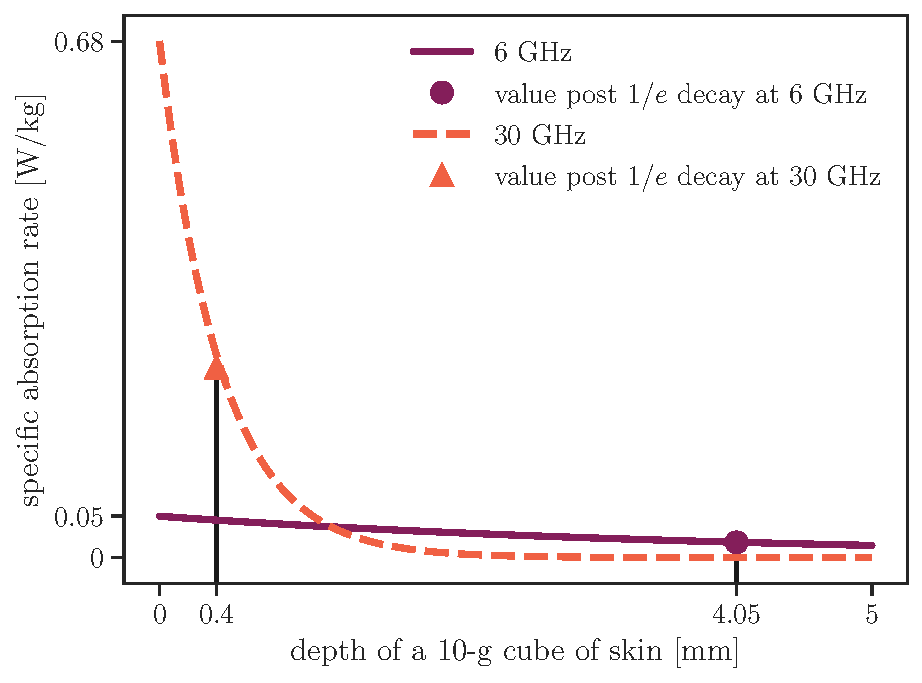
\includegraphics[width=0.8\textwidth]{artwork/sar_decay.pdf}
    \caption{Specific absorption rate as a function of depth into the homogeneous block of tissue with dielectric properties of dry skin. It is assumed that the model is exposed by a plane wave with power density of \SI{1000}{\watt\per\meter\squared}.}
    \label{fig:sar_decay}
\end{figure}
Thus, it is more appropriate to describe absorbed power over surface area.
At \SI{6}{\GHz}, \gls{br} for local exposure are expressed by means of the \gls{apd} as the most of the power is absorbed in the upper portion of a 10-g \gls{sar} cubic volume.
For dry skin of the average density of \SI{1109}{\kg\per\m\cubed}, the cube volume corresponds to \SI{2.15}{\cm\cubed}.
Recent thermal modeling~\cite{Hashimoto2017On} and analytical studies~\cite{Foster2017Thermal} suggest that at the \SIrange[range-units=single,range-phrase=--]{6}{30}{\GHz} range, the exposure over a square averaging area of \SI{4}{\cm\squared}, which matches the area of the front surface of 10-g cube, provides a good correlation for local maximum temperature rise.
This is further supported by simulations of realistic exposure scenarios~\cite{He2018RF}.
To account for narrow beam formation at higher frequencies, the \gls{apd} should be computed on the most exposed area of \SI{1}{\cm\squared} at the \SIrange[range-units=single,range-phrase=--]{30}{300}{\GHz} range.
This ensures that the operational adverse health effect thresholds are not exceeded over smaller regions provided that it does not exceed 2 times the value for the averaging area of \SI{4}{\cm\squared}~\cite{Foster2016Thermal}.
The \gls{apd} of \SI{200}{\W\per\m\squared} averaged over 6-min interval and \SI{4}{\cm\squared} surface area of the exposed region on the body corresponds to the operational adverse health effect threshold for bot the head/torso and limb region.
As with \gls{sar}, a factor of either 2 or 10 is additionally applied as a precautionary measure for occupational exposure or the general public, respectively.

\Gls{br}s for rapid temperature rise after a brief exposure are defined by means of the \gls{sa} at the \SI{400}{\MHz} to \SI{6}{\GHz} range as a function of time.
Much like \gls{sar}, \gls{sa} is spatially averaged over a 10-g cubic mass.
Concrete formulations and values are available elsewhere, e.g. in~\cite{ICNIRP2020Guidelines,IEEE2019Standard}.
An additional safety factor of 2 or 10 is applied to \gls{sa} for occupational exposure or the general public, respectively, to account for scientific uncertainty as well as variability of environmental conditions, physical activity levels, and thermal physiology across the population.

Above \SI{6}{\GHz}, following the same reasoning as for the case of setting \gls{br}s for local steady-state temperature rise, the absorbed energy density is averaged over a square \SI{4}{\cm\squared} area of the most exposed body region of interest.
To account for focal beam exposure at the \SIrange[range-units=single,range-phrase=--]{30}{300}{\GHz} range, averaging should be performed additionally over a square \SI{1}{\cm\squared} area whereas the absorbed energy density should be at most twice the value for a square \SI{1}{\cm\squared} averaging area.
Again, safety factors of 2 and 10 are respectively applied for occupational exposure and the general public, respectively.

\subsection{Exposure Reference Levels}
\Gls{rl}s/\gls{erl}s (from now on in the text only ``\gls{rl}'' abbreviation will be used for the sake of brevity and improved readability) have been derived from a combination of computational and measurement studies to provide more practical means of demonstrating compliance using physical quantities that are easy to assess without the need of having a human body in the measurement loop.
The measurement takes place in free space, where instead of absorbed, incident values are taken into consideration.
In the relevant literature, the term ``exposure assessment'' refers to the evaluation of the level of \gls{rf} \gls{em} energy incident on the exposed body, while ``dosimetry'' refers to determining the absorption of \gls{rf} \gls{em} energy within that body~\cite{Chou1996Radio}.
As incident fields do not undergo any losses caused by the interaction with the body, \gls{rl}s are always more conservative in practice than the corresponding \gls{br}.

The quantities used for specifying \gls{rl} are the \gls{Einc}, \gls{Hinc}, \gls{ipd}, plane-wave equivalent \gls{ipd}, \gls{Uinc}, and \gls{Ueq}, measured outside the body, and electric current inside the body.
Important to consider is to how well the aforementioned physical quantities serve to predict the corresponding physical quantities used to assess compliance with the \gls{br}s.
The accuracy of predictions is strongly related to whether external \gls{em} fields can be considered to be within the far-field, radiative near-field or reactive near-field zone.
Additional confounding variables are the frequency, physical dimensions of the source of external \gls{em} fields, separation distance between the source and body, etc.
Taking all this into consideration, both the \gls{icnirp} guidelines~\cite{ICNIRP2020Guidelines} and \gls{ieee} standard~\cite{IEEE2019Standard} have more conservative, but slightly different rules for exposure in the reactive and near-field than far-field zone~\cite{Hirata2020Difference}.

In this work, the emphasis is the exposure to \gls{rf} \gls{em} waves at the \SIrange[range-units=single,range-phrase=--]{6}{300}{\GHz} range, details for determination of \gls{rl}s out of this range can be found elsewhere, e.g., in chapter ``Reference levels'' of \gls{icnirp}'s 2020 guidelines~\cite{ICNIRP2020Guidelines} and chapter 4.3 ``\gls{drl}s and \gls{erl}s for exposure to electromagnetic fields -- Thermal effects (\SI{100}{\kHz} to \SI{300}{\GHz})'' in the \gls{ieee} C95.1-2019 standard~\cite{IEEE2019Standard}.
At the \SIrange[range-units=single,range-phrase=--]{6}{300}{\GHz} range, the \gls{ipd} is defined as the \gls{rl} averaged during 6-min interval for local exposure either as peak value (at \SI{6}{\GHz}) or spatially-averaged over any exposed \SI{4}{\cm\squared} area in the shape of square (above \SI{6}{\GHz}).
Additionally, at and above \SI{30}{\GHz}, the \gls{ipd} must be averaged over a square \SI{1}{\cm\squared} projected body surface with the restriction it cannot be twice as large compared to the corresponding \SI{4}{\cm\squared} area.

At \SI{6}{\GHz}, within the far-field zone, compliance is demonstrated if the peak spatial \gls{ipd} does not exceed prescribed value.
The plane-wave equivalent \gls{ipd} can be used to substitute the peak spatial \gls{ipd} when appropriate.
Within the radiative near-field zone, compliance is assessed only by using thepeak spatial \gls{ipd}.
Finally, in the reactive near-field zone, \gls{rl}s cannot be used to demonstrate compliance -- \gls{br}s must be assessed in this case.
The same logic applies above \SI{6}{\GHz} and up to \SI{300}{\GHz} where instead of the peak spatial value, the spatially averaged \gls{ipd} is used to demonstrate compliance with prescribed limits.
A detailed overview of \gls{rl} for local exposure, averaged over 6-min interval at the \SIrange[range-units=single,range-phrase=--]{6}{300}{\GHz} range can be found in \cref{tab:rls}.
\begin{table}[ht]
\begin{center}
\caption{(Exposure) reference levels averaged over 6-min interval at the \SIrange[range-units=single,range-phrase=--]{6}{300}{\GHz} range.}
\label{tab:rls}
\resizebox{\textwidth}{!}{%
\begin{tabular}{|c|c|c|cc|}
\hline
\cellcolor[HTML]{EFEFEF} & \cellcolor[HTML]{EFEFEF} & \cellcolor[HTML]{EFEFEF} & \multicolumn{2}{c|}{\cellcolor[HTML]{EFEFEF}{\color[HTML]{333333} value${}^{*}$ [\SI{}{\watt\per\m\squared}]}} \\ \cline{4-5} 
\multirow{-2}{*}{\cellcolor[HTML]{EFEFEF}\begin{tabular}[c]{@{}c@{}}exposure\\ scenario\end{tabular}} & \multirow{-2}{*}{\cellcolor[HTML]{EFEFEF}frequency [GHz]} & \multirow{-2}{*}{\cellcolor[HTML]{EFEFEF}\begin{tabular}[c]{@{}c@{}}(exposure)\\ reference levels\end{tabular}} & \multicolumn{1}{c|}{ICNIRP~\cite{ICNIRP2020Guidelines}} & IEEE~\cite{IEEE2019Standard} \\ \hline
 & 6 &  & \multicolumn{1}{c|}{200} & 200 \\ \cline{2-2} \cline{4-5} 
 & 6--300 &  & \multicolumn{1}{c|}{$275 \; f_G^{-0.177}$} & $274.8 \; f_G^{-0.177}$ \\ \cline{2-2} \cline{4-5} 
\multirow{-3}{*}{\begin{tabular}[c]{@{}c@{}}occupational\\ (restricted\\ environments)\end{tabular}} & 300 &  & \multicolumn{1}{c|}{100} & 100 \\ \cline{1-2} \cline{4-5} 
 & 6 &  & \multicolumn{1}{c|}{40} & 40 \\ \cline{2-2} \cline{4-5} 
 & 6--300 &  & \multicolumn{1}{c|}{$55 \; f_G^{-0.177}$} & $55 \; f_G^{-0.177}$ \\ \cline{2-2} \cline{4-5} 
\multirow{-3}{*}{\begin{tabular}[c]{@{}c@{}}general public\\ (unrestricted\\ environment)\end{tabular}} & 300 & \multirow{-6}{*}{\gls{ipd}} & \multicolumn{1}{c|}{20} & 20 \\ \hline
\end{tabular}%
}
\end{center}
${}^{*}f_G$ stands for the frequency in \SI{}{\GHz}.
\end{table}

Furthermore, to put values in the visual frame of reference, in \cref{fig:reference_levels}, the \gls{ipd} as a function of frequency is shown over the \SIrange[range-units=single,range-phrase=--]{6}{300}{\GHz} range.
\begin{figure}[ht]
    \centering
    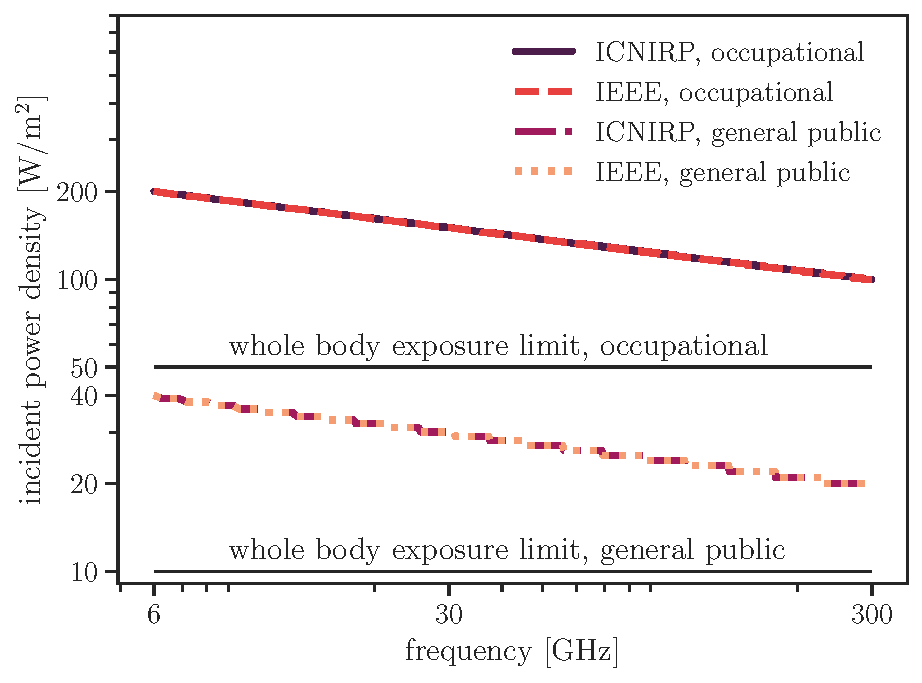
\includegraphics[width=0.8\textwidth]{artwork/reference_levels.pdf}
    \caption{Reference levels for occupational exposure and general public averaged over 6-min interval at the \SIrange[range-units=single,range-phrase=--]{6}{300}{\GHz} range. Both \gls{icnirp} and \gls{ieee} curves for the \gls{ipd} as a function of the frequency are shown to demonstrate harmonization between prescribed limits. Additionally, black horizontal lines show (exposure) reference levels for whole body exposure over 30-min interval at constant values of \SI{10}{\watt\per\m\squared} and \SI{50}{\watt\per\m\squared} for general public and occupational exposure, respectively.}
    \label{fig:reference_levels}
\end{figure}
\Gls{rl}r for whole-body exposure are also shown both for occupational exposure and general public and are set to constant values of \SI{50}{} and \SI{10}{\watt\per\m\squared}, respectively.
As for local exposure, at \SI{6}{\GHz} within the far-field zone, compliance is demonstrated if the peak spatial \gls{ipd} does not exceed the prescribed value where, if appropriate, the plane-wave equivalent \gls{ipd} can be used instead of the \gls{ipd}.
In the radiative near-field zone, compliance is demonstrate only if the \gls{ipd} does not exceed the limits.
Finally, within the reactive near-field zone, compliance cannot be demonstrated by using the \gls{ipd} and the corresponding dosimetric value must be assessed.

In cases of simultaneous exposure to multiple frequency \gls{rf} \gls{em} fields, it is important to evaluate whether these exposures are additive in their effect.
This cumulative effect should be treated separately for the thermal and electrical stimulation, and restrictions should be set accordingly.
This issue is out of the scope of this document.
Details can be found elsewhere, e.g., in~\cite{ICNIRP2020Guidelines, IEEE2019Standard}.
However, it is noteworthy that in~\cite{Miura2021Power}, simultaneous exposure is evaluated at \SI{2}{} and \SI{28}{\GHz} by evaluating power absorption and skin temperature rise in the near-field zone of realistic antenna models.
It is demonstrated that the effect of superposition is marginal in all cases except when the patch antenna array and inverted-F antenna are separated by less than \SI{50}{\mm} at \SI{5}{\mm} antenna-body separation.
